
\chapter{语言建模实验结果与分析}
前面两章分别介绍了基于树状和类别的层次概率模型的具体建模过程,本章将比较这两种分层模型与已有的算法(Baselines)在计算效率和精确性上的差异,并且在三个标准文本数据集上进行语言建模的实验研究和结果分析。
接下来将讨论分析不同层次概率算法与其他大词表问题的优化算法在单词困惑度和单词错误率上的结果对比和实验分析。除此以外,还将从效率、可扩展性、参数大小等方面对这些方法进行实验研究并作讨论分析。

\section{实验设置}
这一小节将介绍实验所需要用到的文本数据集,还有语言建模实验的两种主要的评测指标和实验模型的实际参数配置和训练过程。
\subsection{实验数据集}
本实验所采用的数据集主要是依照两个目的选取:1)首先为了便于实验复现和互相对比,需要在小数据集上反映出参数变化对模型最后的性能产生的影响;2)同时还需要在大数据集上展示模型参数在最佳参数配置下,比较模型之间的最优结果的差异点。
所以本实验选取了三个标准文本数据集:Wikitext-2,Wikitext-103 和 One Billion Words(OBW)数据集。
如表~\ref{tab:dataset}~所示,表中列举了这三个数据集的相关统计指标,包括:单词数量、句子数量、词表大小和词表外单词的比例(Out-of-Vocabulary,OOV)。需要注意的是词表大小不能改变,因为不同词表规模的模型之间理论上就不在同一个基准之上,其次是由于模型的一个的评测指标和词表大小成负相关关系,所以表~\ref{tab:dataset}~中展示的数据已经预先固定不会再做任何的修改,例如:不能对数据集做单词大小写变化、数词转换操作或者分词操作。
\begin{table}[!ht]
  \centering
  \caption{WikiText-2、WikiText-103 和 One Billion Words 数据集统计指标 \label{tab:dataset}}
\begin{tabular}{llrrrrr}
\toprule
数据集& 类型& 文章数量  & 句子数量 & 单词数量 & 词表大小 & OOV(\%) \\ \midrule
\multirow{3}{*}{Wikitext-2} &训练集& 600 & 36,718 & 2,088,628 & \multirow{3}{*}{33,278} & \multirow{3}{*}{2.6\%} \\
&验证集& 60 &3,760 & 217,646  & &\\
&测试集& 60 & 4,358 & 245,569 & &\\
\midrule
\multirow{3}{*}{Wikitext-103} &训练集& 28,475 &  1,801,350 &  103,227,021 & \multirow{3}{*}{267,735} & \multirow{3}{*}{0.4\%} \\
&验证集& 60 &3,760 & 217,646  & &\\
&测试集& 60 & 4,358 & 245,569 & &\\
\midrule
\multirow{3}{*}{One Billion Words} &训练集& --- &30,301,028&768,646,526&   \multirow{3}{*}{793,471} &   \multirow{3}{*}{0.28\%} \\
 &验证集& --- &  6,075 &   153,583 &&\\
 &测试集 & --- &  6,206 &   159,354 &&\\
\bottomrule
\end{tabular}
\end{table}

Wikitext-2~和~Wikitext-103~数据的训练集(Training Dataset)、验证(Validation Dataset)和测试集(Testing Dataset)都是预先划分固定的,并且其词表大小也已经被定义\footnote{https://metamind.io/research/the-wikitext-long-term-dependency-language-modeling-dataset/}。
这两个数据集的验证集和测试集是相同的,而~Wikitext-103~的训练集大小则是~Wikitext-2~的训练集的50倍左右,所以还可以间接测算出增大训练集对测试集预测准确率的提升效果。
对于第三个``One Billion Words''数据集\footnote{http://www.statmt.org/lm-benchmark/},它是由历史机器翻译数据集积累的文本融合而成,文本数据也取自维基百科(Wikipedia)\footnote{https://en.wikipedia.org/wiki/Main\_Page/}。
为了保证评价的准确性性和实验的可互比性,官方提供了一套数据预处理脚本,同时指定了该脚本所需要的~Perl~语言版本,要求极为严苛。
因为对于文本数据来说,Perl~内置函数版本不同处理出来的文本也略有不同,语言模型之间的结果就不在同一个基准之上。
当用官方提供的脚本处理完数据后,我们将``./train/''目录中所有数据视为训练集,选择``./holdout/''目录下第一和第二个数据集作为相应的验证和测试集,这些数据集的详细统计指标在表~\ref{tab:dataset}~中进行了说明。

\subsection{实验评价指标}
当实验模型在验证数据集上收敛后就需要评价不同模型的性能差异,本实验考虑语言模型的两个评估度量标准:困惑度(Perplexity,$ \mathrm{PPL} $)和单词误差率(Word Error Rate,$\mathrm{WER} $),来比较和评估不同的优化方法的差异和优劣。
其中,$\mathrm{PPL}$~是一种内在度量指标(Intrinsic Metric),代表了在不同语境中选择下一个候选单词时的困惑程度。语言模型困惑度较低,意味着在相同词表下模型拥有更好的可预测性。
此外在整个测试集上,$\mathrm{PPL}$~数值是与模型的代价函数($\ell$)呈指数相关关系,这表明训练过程中模型直接优化了~$ \mathrm{PPL} $~评测指标,其数学定义如下所示:
\begin{equation}\label{equ:ppl}
   \mathrm{PPL}(w_1,\cdots,w_T)=\sqrt[T]{\frac{1}{\prod_{t=1}^T p(w_t|w_{1:t-1})}}
\end{equation}

此外,$\mathrm{WER}$~表示单词的萊文斯坦距离(Levenshtein Distance),用于衡量参考句子(Reference,记作r)和预测句子(Hypothesis,记作h)之间的相似度。它是编辑距离的一种衍生类型,被定义为错误识别的单词(删除,插入,替换)占总单词的百分比\footnote{https://martin-thoma.com/word-error-rate-calculation}:
\begin{equation}\label{equ:wer}
  \mathrm{WER} = \frac{\text{插入的单词数 + 删除的单词数 + 替换的单词数}}{\text{全部单词数量}}
\end{equation}
计算错误识别的单词的方法如下所示:
\begin{equation}\label{equ:distance}
d_{r,h}(i,j)=\begin{cases}
\max (i,j)& \text{如果}\min(i,j)=0\\
\min  \begin{cases}
d_{r,h}(i-1,j)+1,\text{//插入的单词}\\
d_{r,h}(i,j-1)+1,\text{//删除的单词}\\
d_{r,h}(i-1,j-1)+1\{r_i\neq h_j\}.\text{//替换的单词}
\end{cases} &\text{否则}
\end{cases}
\end{equation}
其中~$1\{r_i\neq h_j\}$~指代的是示性函数,当且仅当~$r_i= h_j$~的时候取值为~$0$,否则该函数取值为~$1$。 $d_{r,h}(i,j)$~表示参考句子~$r$的第~$i$~个字符与预测句子~$r$~第~$j$~个字符之间的距离,同时萊文斯坦距离满足度量的延展性关系(三角不等式),即: 两个字符串的距离不大于分别与第三个字符串的距离之和:
\begin{equation}
d_{r,h}+d_{r,s}\ge d_{r,s}
\end{equation}
公式中的~$s$~代表另外一个生成的句子,$d_{r,h}$~表示句子~r~和句子~h~之间的编辑距离。

除了以上的定量指标外,本实验还考虑了``训练时间效''、``词表可伸缩性''~和~``运行时内存消耗''这三个不同的定性指标,作为评估不同模型的性能的重要依据。

\subsection{模型训练和参数配置}
接下来介绍实验模型所涉及的参数设置和训练过程。在具体算法实现中,每个模型都是使用~Theano~框架实现,而且都运行在一个独立的显卡设备上,模型不在多显卡上运算,模型训练过程不互相干扰。
本实验采用的显卡具有~12GB~的显存(设备型号是~Nvidia K40m),保证能进行大矩阵乘法的运算,所以能测算出大词表问题的具体计算代价。实验发现模型的内存占用量在试验中随着参数维数的增加而快速增长,单个显卡的显存资源被快速利用殆尽。

然后是针对数据集做必要的预处理。对于~Wikitext-2~数据集,最大句子长度固定为~256;对于~Wikitext-103~数据集,最大句子长度固定为~100;对于~OBW~数据集,最大句子长度固定为~50。因为第三个数据集的词表最大,需要占用更多的显存资源,所以句子长度有所缩减,以减少计算过程中的二维矩阵或者三维张量占据过多空间。
长度超过阈值的那部分字符串将被直接删除,由于语言模型测量的是单词级损失(Word-Level Loss)而不是句子级的分数(Sentence-Level Loss),因此删除部分的句子对模型训练的影响很小。

\begin{figure}[!t]
  \centering
  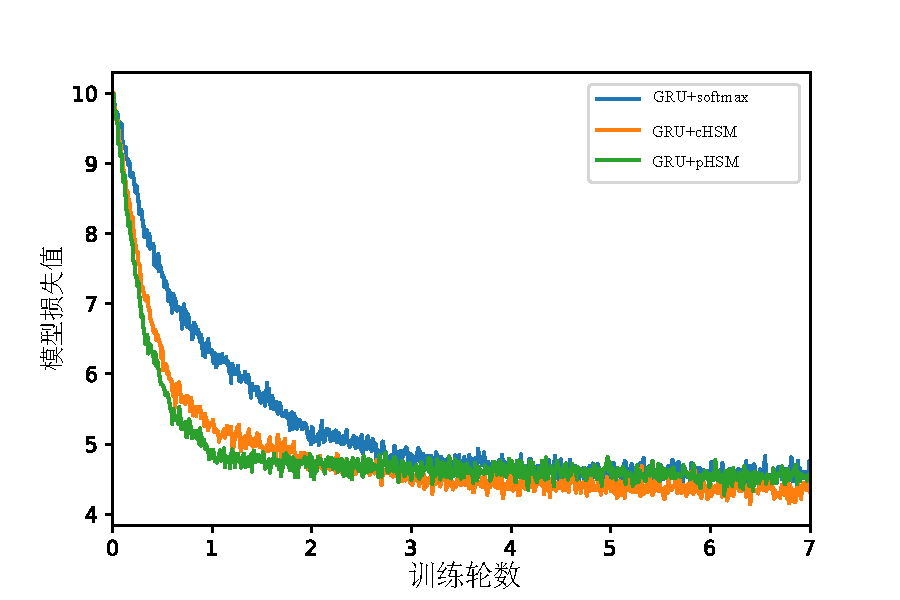
\includegraphics[width=0.6\columnwidth]{./figures/learn2.pdf}
  \caption{模型训练曲线图}
\end{figure}

另外,本实验采用~Adam~算法(Optimizer)配合两种初始学习率(Learning Rate)作为模型的优化求解函数,即设置~$\mathtt{lr}=0.06$~和~$0.001$。两种词表层次分解方法收敛速度较慢需要采用较大的学习率,而传统的softmax和采样近似方则需要采用较小的学习率。除此以外,为了减弱模型收敛过程中的损失值的振荡现象,每隔一定步数($\texttt{Step} =100$),学习率还需要逐渐缩小:$\texttt{lr}\leftarrow\texttt{lr}*0.9$。

对于在~Wikitext-2~数据集上运行的实验,设置批处理大小(Batch Size)为~20~并且最大遍历周期(Epoch)为~15。当模型在验证集上收敛后,验证集损失值大约在 4.8左右。
而~Wikitext-103~数据集设置的最大遍历周期(Epoch)大约为~5-10~个轮数,Wikitext-103~训练集大约是~Wikitext-2~的~50~倍需要的遍历周期相对更少。
当模型在验证集上收敛后,验证集损失值大约在~5.1~左右,Wikitext-103~的词表相对更大导致模型的预测困惑度更高。
实验发现~Wikitext-2~和~Wikitext-103~的唯一区别是训练数据的大小,增大训练数据集不一定能保证模型在相同的验证和测试集上结果更好,因为训练数据训练集增大~50~倍的同时词表也增大了~3~倍。

此外,在~OBW~数据集上运行的实验需要更大的参数集合来拟合导致计算缓慢同时收敛也缓慢。
为了减少计算时间,本实验应用~CuDNN~实现的~RNN~模型~\upcite{DBLP:journals/corr/AppleyardKB16},这将会把~RNN~部分所需要的计算时间降到最低,然而实际模型收敛时间也需要大约~480~小时。

\section{影响因素比较}

这部分将讨论语言模型的大词表问题在具体实验中瓶颈和各种不同优化策略对该问题的计算效率和性能的提升和分析。
\begin{figure}[!b]
  \centering
  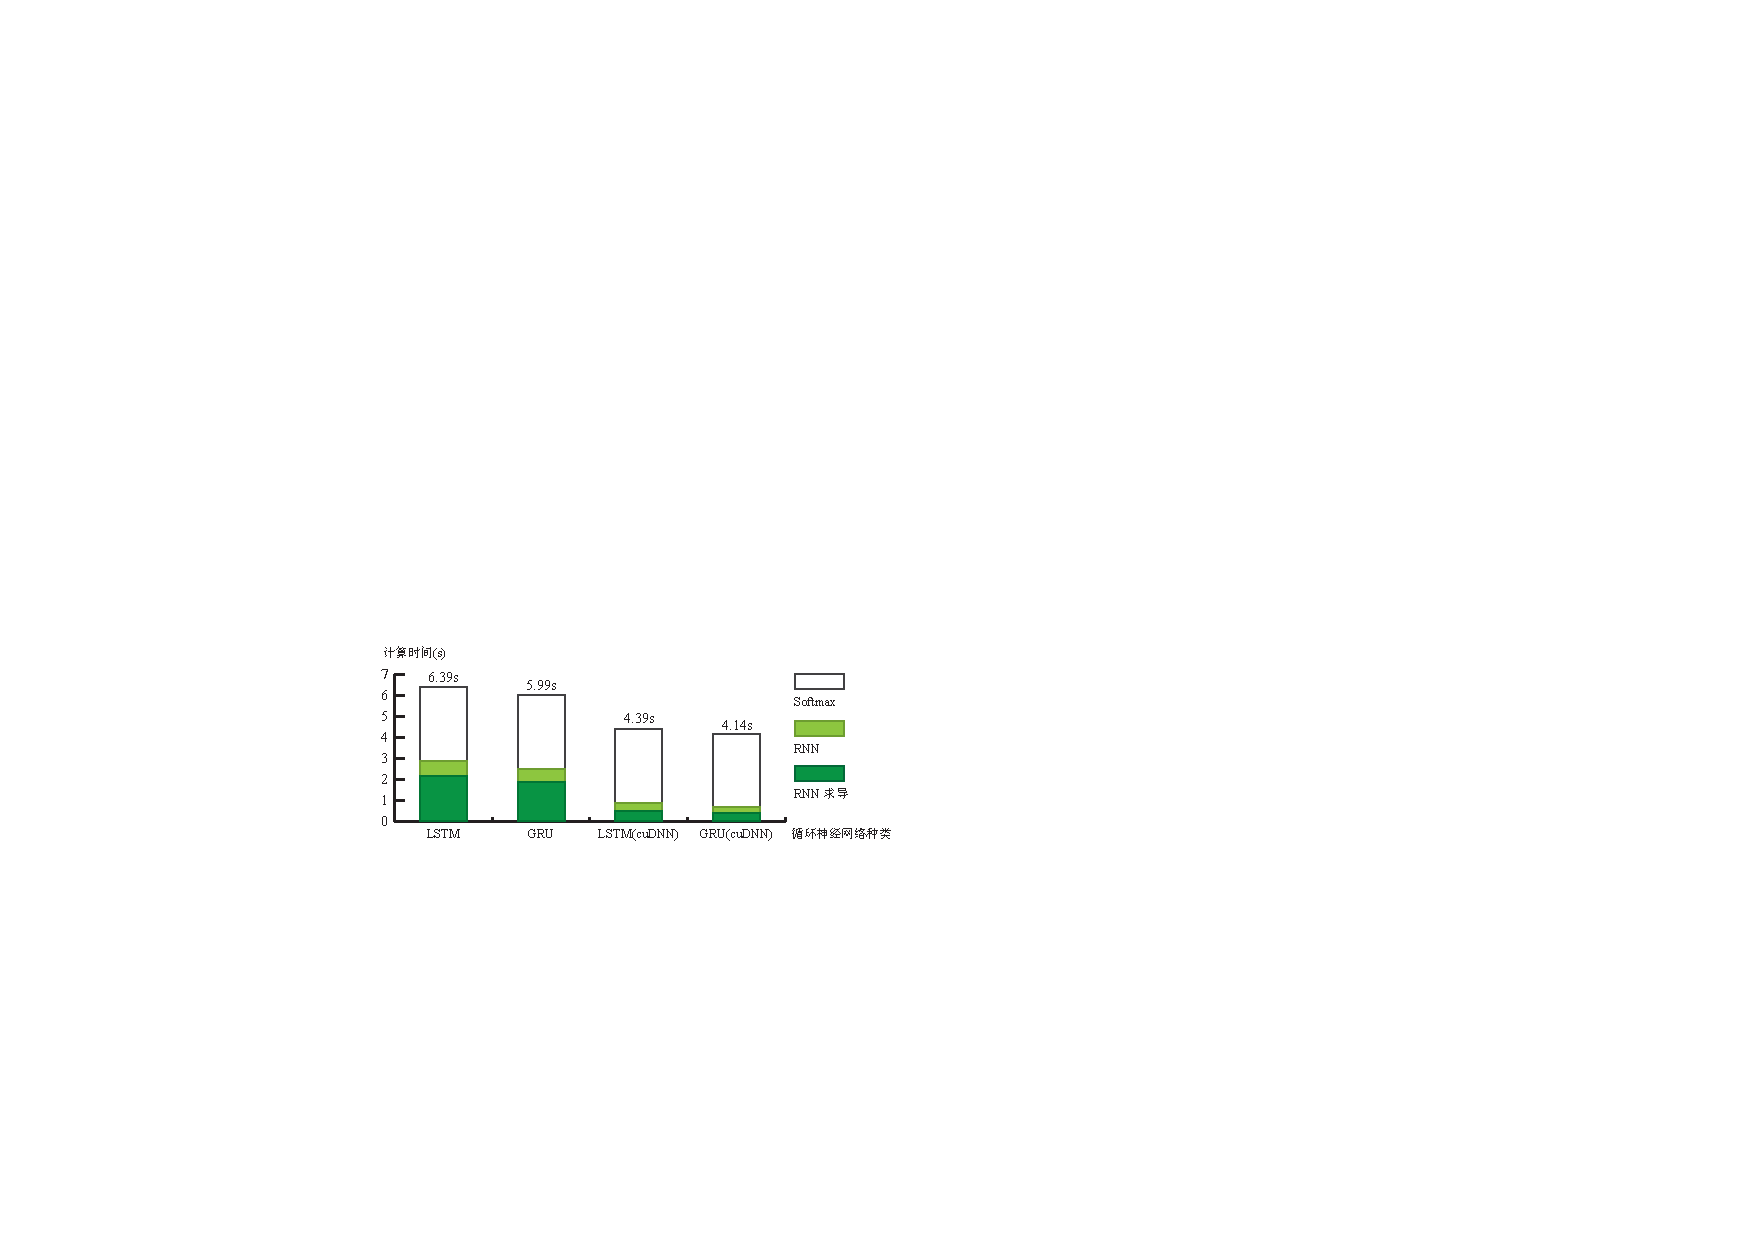
\includegraphics[width=.9\columnwidth]{./figures/rnn_timing.pdf}
  \caption{Wikitext-103数据集上测量语言模型三个部分的计算时间比较}\label{fig:rnn_timing}
\end{figure}
\subsection{大词表问题实验分析}

考虑到~Wikitext-103~数据集的词表大小与平时所采用的数据集的词表相当,本文首先在该数据集上统计了语言模型中每个模块的计算时间消耗,统计softmax函数、不同的RNN结构(即LSTM~模型和~GRU~模型)及其梯度(即,RNN Gradient)所需的时间,如图~\ref{fig:rnn_timing}~所示。
我们分别用~Theano~框架和~CuDNN~实现了~RNN~模块,前两组采用~Python~语言实现,后两组的RNN模块的核心计算部分使用~C++~语言实现,同时采用~Python~完成调用的封装函数。目前基于~CuDNN~实现的~RNN~模型计算时间最快,保证~RNN~模块的运行时间可以缩减到最短。 我们将实验重复了~100~遍并统计每个模块的平均占用的时间消耗,其目的是通过多次实验来保证实验数据准确性并减少随机误差。


从图~\ref{fig:rnn_timing}~中可以看出,使用基于~CuDNN~实现的~RNN~模块之后,softmax~模块占用的时间远超过总时间的~80\%并且~softmax~函数计算时间占比随着词表的增大而越来越大,这就需要我们详细讨论~softmax~函数的优化。


\subsection{词表层次化比较}
表~\ref{tab:time}~中统计了不同层次概率模型在~WikiText-103~数据集上的平均计算时间消耗。
其中输入句子的最大长度是$50$,隐藏层维度为$256$,输出端的词表大小是$267735$和批量处理大小设置为 20。此外,``总计算时间''表示模型的前向概率计算和后向梯度优化的过程,``前向计算时间 ''表示从输入数据到计算模型代价函数所消耗的时间,同时还给出了不同算法在训练中的内存占用。$\mathcal{|V|}$~表示词表大小,$\mathcal{|H|}$~是隐藏层维度。

由该表分析可知,在训练训练过程中tHSM算法消耗最小的内存,而p-tHSM算法需要消耗相对较大的内存。同时p-tHSM算法在三类统计项中计算速度都是最高的,只有在GPGPU配置的代价函数计算环节比cHSM算法慢。

\begin{table}[!ht]
  \centering
  \caption{Wikitext-103数据集上GPGPU和CPU的运行时内存和计算时间比较\label{tab:time}}
\begin{tabular}{lccccc}
  \toprule
 \multirow{2}{*}{算法}  &\multirow{2}{*}{运行时内存占用} &\multicolumn{2}{c}{总计算时间 (ms)} & \multicolumn{2}{c}{前向计算时间 (ms)}   \\
   \cmidrule(lr){3-4}  \cmidrule(lr){5-6}
	& & CPU&GPGPU & CPU& GPGPU \\ \midrule
Softmax & $\mathcal{|HV|}$ &510.4  &262.1&352.2& 62.9 \\
cHSM    & $2\mathcal{|H|\sqrt{|V|}}$&506.5  &\textbf{40.6}&28.7&14.6 \\
tHSM    &$\mathcal{|H|}$&1,004.0 &444.4 & 8.1&  5.6   \\
p-tHSM  &$\mathcal{|H|\log{|V|}}$ &\textbf{383.5}&	86.4 &\textbf{7.0}&	\textbf{1.4} \\
  \bottomrule
\end{tabular}
\end{table}

\begin{figure}[!t]
  \centering
  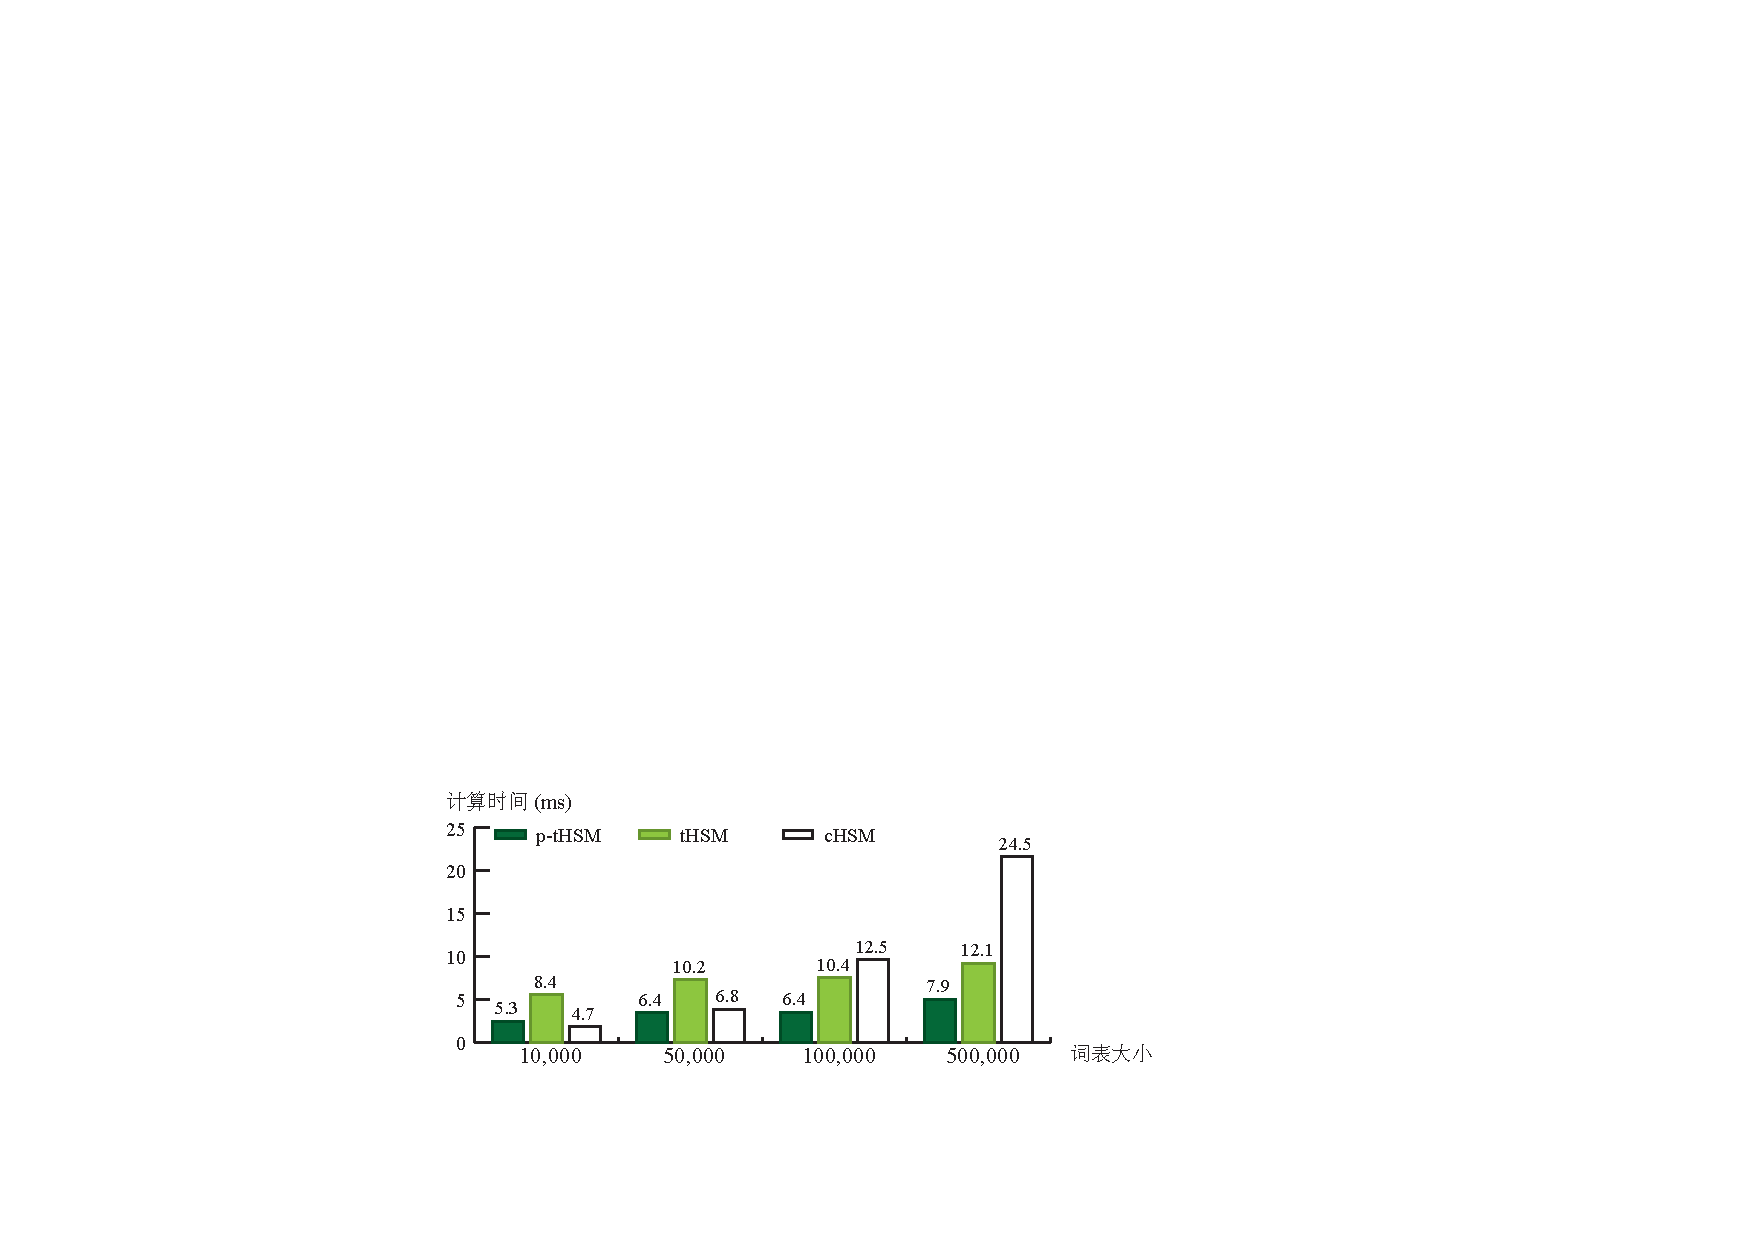
\includegraphics[width=.87\columnwidth]{./figures/all_time.pdf}
  \caption{cHSM、tHSM 和 p-tHSM 算法随着词表大小的计算时间影响}\label{fig:hsm_benchmark}
\end{figure}

\subsection{词表伸缩性比较}
图~\ref{fig:hsm_benchmark}~验证cHSM、tHSM和p-tHSM算法对词表大小的伸缩性的实验结果,这里不包``softmax''方法,因为与其他算法相比,它消耗相当多的计算时间无法被放在这个图里面。 从图中分析得知,cHSM计算时间与词表的平方根呈线性关系(即,$\mathcal{O(\sqrt{|V|})}$),tHSM算法的计算时间与词表的对数成线性关系 (即,$\mathcal{O(\log{|V|})}$)。同时本论文中提出的p-tHSM算法的计算效率相比于tHSM算法更高。这是由于是传统tHSM算法需要逐个访问树的节点对应的参数向量,花费了部分时间在矩阵的Indexing操作中,而本文提出的算法则直接将路径上所有的参数向量加载进内存直接避免了该Indexing操作,从而达到了计算效率的提升。
%在这些实验的基础上,我们可以得出结论:所提出的p-tHSM方法胜过历史记录~$\mathcal{O(|H|\log|V|)})$,并且取得了令人满意的分层softmax方法的加速比。 这种性能归因于基于GPGPU并行性的加速,也是由于p-tHSM 方法的基本结构,能够将目标字树进行并行地计算。


\subsection{搜索策略的影响}
接下来分析模型在测试过程中的不同的搜索策略对实验指标WER的影响,如表~\ref{tab:search}~和表~\ref{tab:search}~所示。


算法~\ref{alog:global}~表示先计算所有单词的得分然后再做排序。对于~p-tHSM~算法,我们比较了所提出的算法~\ref{alog:greed_argmax}~和传统的算法~\ref{alog:global}在计算速度和准确度上的实验分析。算法~\ref{alog:greed_argmax}~比算法~\ref{alog:global}~方法计算结果花费的时间更少。由于基于树的模型在逐层访问路径的过程中更容易出现错误情况,所以算法~\ref{alog:global}~的WER分数比算法~\ref{alog:greed_argmax}~相对更好。
\begin{table}[!ht]
  \centering
  \caption{Wikitext-2数据集上~p-tHSM~算法针对不同搜索算法的WER评测结果\label{tab:search}}
\begin{tabular}{ccccc}
  \toprule
     层次概率模型   & 算法类别&计算时间(ms)&验证集(WER)& 测试集(WER)\\ \midrule
  \multirow{2}{*}{p-tHSM}  &全局计算(算法~\ref{alog:global})&161& \textbf{76.67\%}&\textbf{75.35\%}\\
        &贪心计算(算法~\ref{alog:greed_argmax})&\textbf{30} & 79.61\%&79.32\%\\
  \bottomrule
\end{tabular}
\end{table}

\begin{table}[!ht]
  \centering
  \caption{Wikitext-2数据集上~cHSM~算法针对不同搜索算法的~WER~评测结果\label{tab:search}}
\begin{tabular}{ccccc}
  \toprule
  层次概率模型 & 算法类别&计算时间 (ms)&验证集(WER)& 测试集(WER)\\ \midrule
  \multirow{3}{*}{cHSM} &全局argmax(算法~\ref{algo:alls})&102& 80.00\%& 80.02\%\\
        &贪心argmax(算法~\ref{alog:exact})&87& 80.00\%& 80.02\%\\
        &伪贪心argmax(算法~\ref{alog:cargmax})&\textbf{44}& 82.09\%&  82.07\%\\
  \bottomrule
\end{tabular}
\end{table}


算法~\ref{alog:exact}~比算法~\ref{algo:alls}~WER指标相同,但是算法~\ref{alog:exact}~计算速度相对较快,这是因为算法\ref{alog:exact}避免了不断调用$p^c$的概率的冗余操作。同时算法~\ref{alog:cargmax}~的计算速度最快,但是损失了模型的预测精度。


\subsection{门限机制的影响}

如表~\ref{tab:rnn}~所示,在 PPL,WER 这两种指标评测中,拥有门控单元的~LSTM~和~GRU~网络比传统的~RNN Relu~和~RNN Tanh~模型表现得更好,这是因为门控单元可以避免循环网络中的梯度消失的问题。在计算时间的评测指标上,传统的网络结构比带有门限机制的网络计算效率更高,同时从表中分析发现~LSTM~比~GRU~模型需要更少的计算时间。这是由于~LSTM~的计算公式中参数的相似性和独立性,我们可以并行计算各个门节点,然而~GRU~模型之间计算步骤存在较大的依赖关系,需要按时序计算,进而LSTM计算速度稍快于GRU模型。

\begin{table}[!ht]
  \centering
  \caption{Wikitext-2数据集上不同循环网络针对 PPL、 WER和计算时间的影响\label{tab:rnn}}
\begin{tabular}{lccc}
  \toprule
  循环神经网络 & 计算时间(ms)&验证集(PPL / WER) & 测试集(PPL / WER)\\ \midrule
  1$\times$RNN Relu~\cite{DBLP:journals/jmlr/GutmannH10} &176.4&260.52 / 80.00\%&238.75 / 80.02\%\\
  1$\times$RNN Tanh~\cite{DBLP:journals/iclr/JiVSAD15}   &176.2&250.57 / 79.61\%&230.98 / 79.32\%\\
  1$\times$LSTM~\cite{7508408}                  &\textbf{189.5}&180.98 / 77.16\%&165.60 / 76.67\%\\
  1$\times$GRU~\cite{DBLP:journals/corr/ChungGCB14}      &191.3&\textbf{179.59 / 77.09\%}&\textbf{165.32 / 77.07\%}\\ \midrule
  2$\times$RNN Relu~\cite{DBLP:journals/jmlr/GutmannH10} &266.3&190.52 / 73.01\%&198.75 / 73.02\%\\
  2$\times$RNN Tanh~\cite{DBLP:journals/iclr/JiVSAD15}   &266.3&189.57 / 72.62\%&260.98 / 72.32\%\\
  2$\times$LSTM~\cite{7508408}                  &\textbf{279.4}&164.98 / 71.17\%&165.60 / 71.67\%\\
  2$\times$GRU~\cite{DBLP:journals/corr/ChungGCB14}      &281.2&\textbf{158.59 / 70.08\%}&\textbf{155.32 / 70.07\%}\\
  \bottomrule
\end{tabular}
\end{table}

\subsection{截断~BPTT~的影响}
接下来分析RNN模型的反向求导模块对实验结果的影响。在~RNN~模型求导数过程中,因为隐藏层是随时间共享的,所以计算导数的时候求导链需要反向传播(Back Propagation Through Time,BPTT)。若是批量数据输入,模型的求导链的计算代价与该批次文本中最长的序列长度相同。考虑到不同批次中的句子长度各异,该求导算法可以通过截断求导链的方式减少模型计算量,该方法被称为截断~BPTT~算法。其优点是模型的各个步骤的损失值计算反向导数的步数是一致的,与句子的长度无关,进而模型的训练速度有所提升。如图~\ref{fig:minibatch}~所示,前向概率计算步骤仍然是相同的,唯一的影响是避免过长的梯度反向传播步骤。


\begin{figure}[!t]
  \centering
  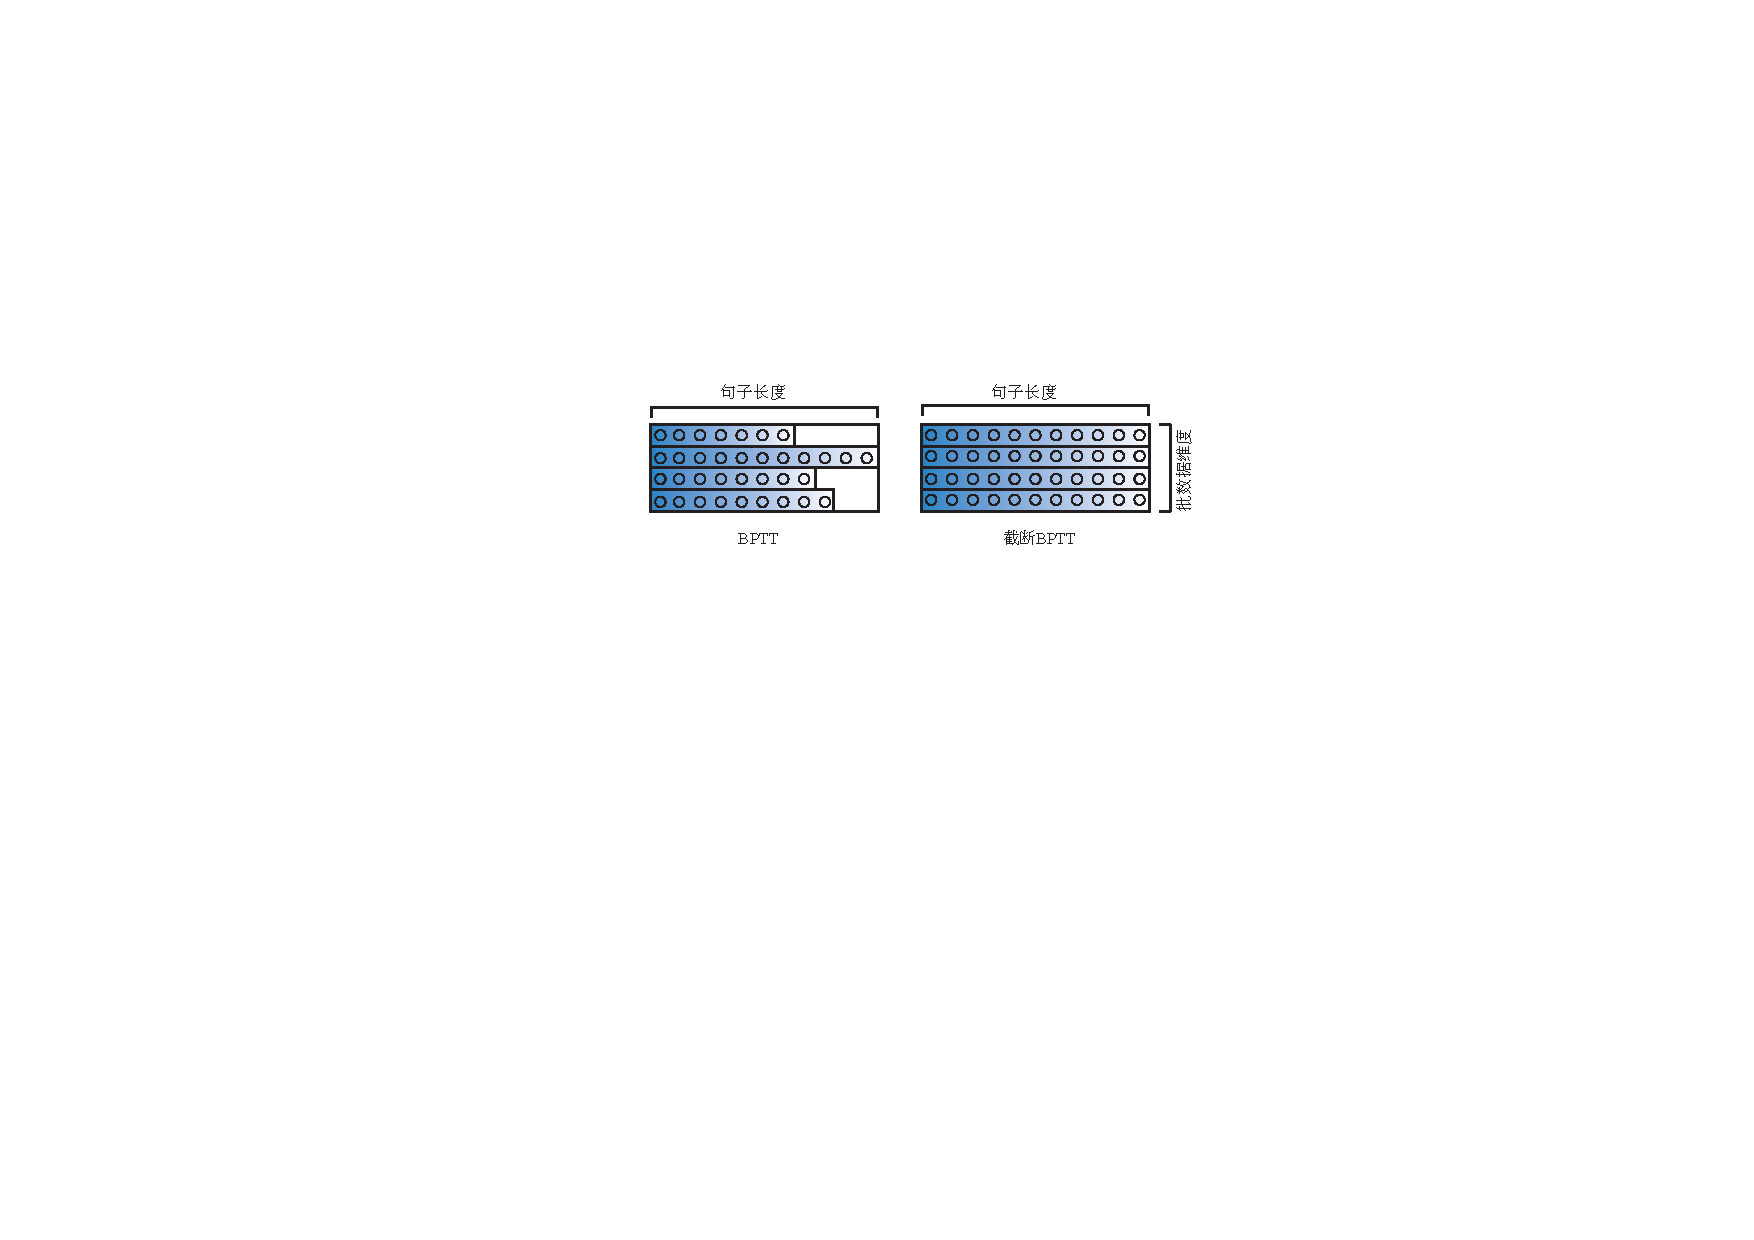
\includegraphics[width=.75\columnwidth]{./figures/minibatch.pdf}
  \caption{BPTT和截断BPTT算法示意图}\label{fig:minibatch}
\end{figure}

其次说明截断~BPTT~操作与文本的长距离依赖之间的关系。在训练过程中,如果依赖关系存在于被截断的语句中,则模型可以学习这种关系; 如果依赖关系总是跨越不同的语句块,那么被截断的语句中不存在这种该依赖关系,从而模型将无法学习这种关系。 其原因是模型的参数导数无法回溯到最初的跨段的那个单词,进而无法更新相应的参数学习这种跨段的依赖关系。
如果这种依赖关系仅存在于单个语句段中,由于模型的参数能求导到前面对应的单词,模型能学习到这种关系。
然而在测试时,模型不存在这个限制,它能在跨语句段中预测这种依赖关系, 因为模型的计算步骤是不断向前传播,不存在模型反向求导的计算过程。
\begin{figure}[!ht]
  \centering
  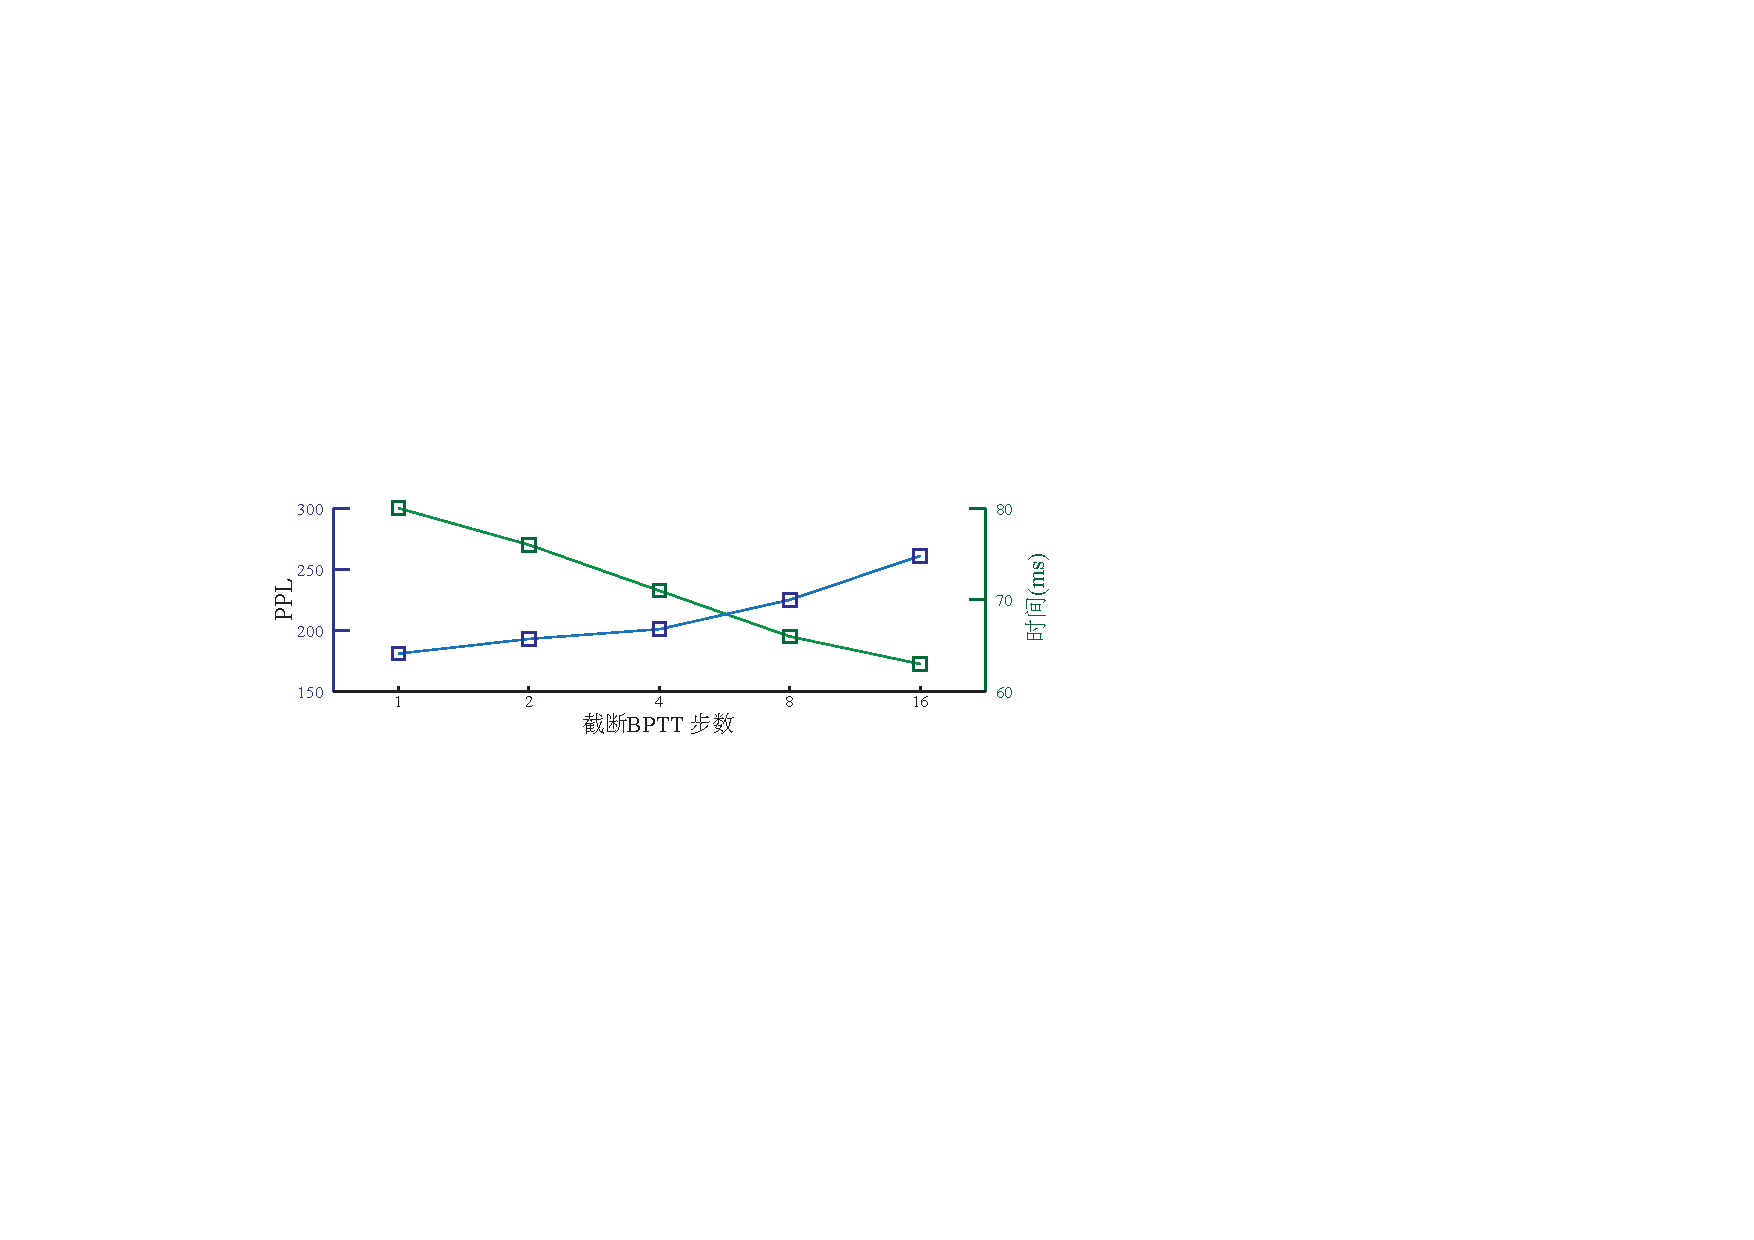
\includegraphics[width=.85\columnwidth]{./figures/tbptt.pdf}
  \caption{Wikitext-2数据集上 BPTT和截断BPTT算法对RNN的影响}\label{fig:tbptt}
\end{figure}

从图~\ref{fig:tbptt}~中可以看出,截断BPTT较小时模型的时间计算速度相对较高同时模型的的PPL数值较高,截断BPTT较大时模型的时间计算速度相对更慢同时模型的的PPL数值较低。


\subsection{采样近似算法比较}
基于采样估计的算法的效率和准确性与样本大小密切相关,从而这小节将评测了两种采样算法的性能。
本实验测试不同采样样本数~$k$~对模型的训练和测试的结果的影响,结果展示在图~\ref{fig:blackout_nce}中。
从图中分析,在平均每次迭代中~Blackout~算法收敛性比传统的~NCE~算法相对更好,但是~NCE~算法计算效率比~Balckout~更高。所以在单位时间中~NCE~算法收敛速度更快,这与~Ji~等人的实验结果是一致的~\upcite{DBLP:journals/iclr/JiVSAD15}。同时在该实验中,当$k=1$时,采样函数计算的就是真正的二元分类概率,此时采样算法振荡现象很剧烈,无法收敛。当逐渐增大采样样本数~$k$,采样算法才能逐渐开始收敛。两种算法的加速比均是~$V/k$,与超参数~$k$~呈负相关关系。

\begin{figure}[!t]
  \centering
  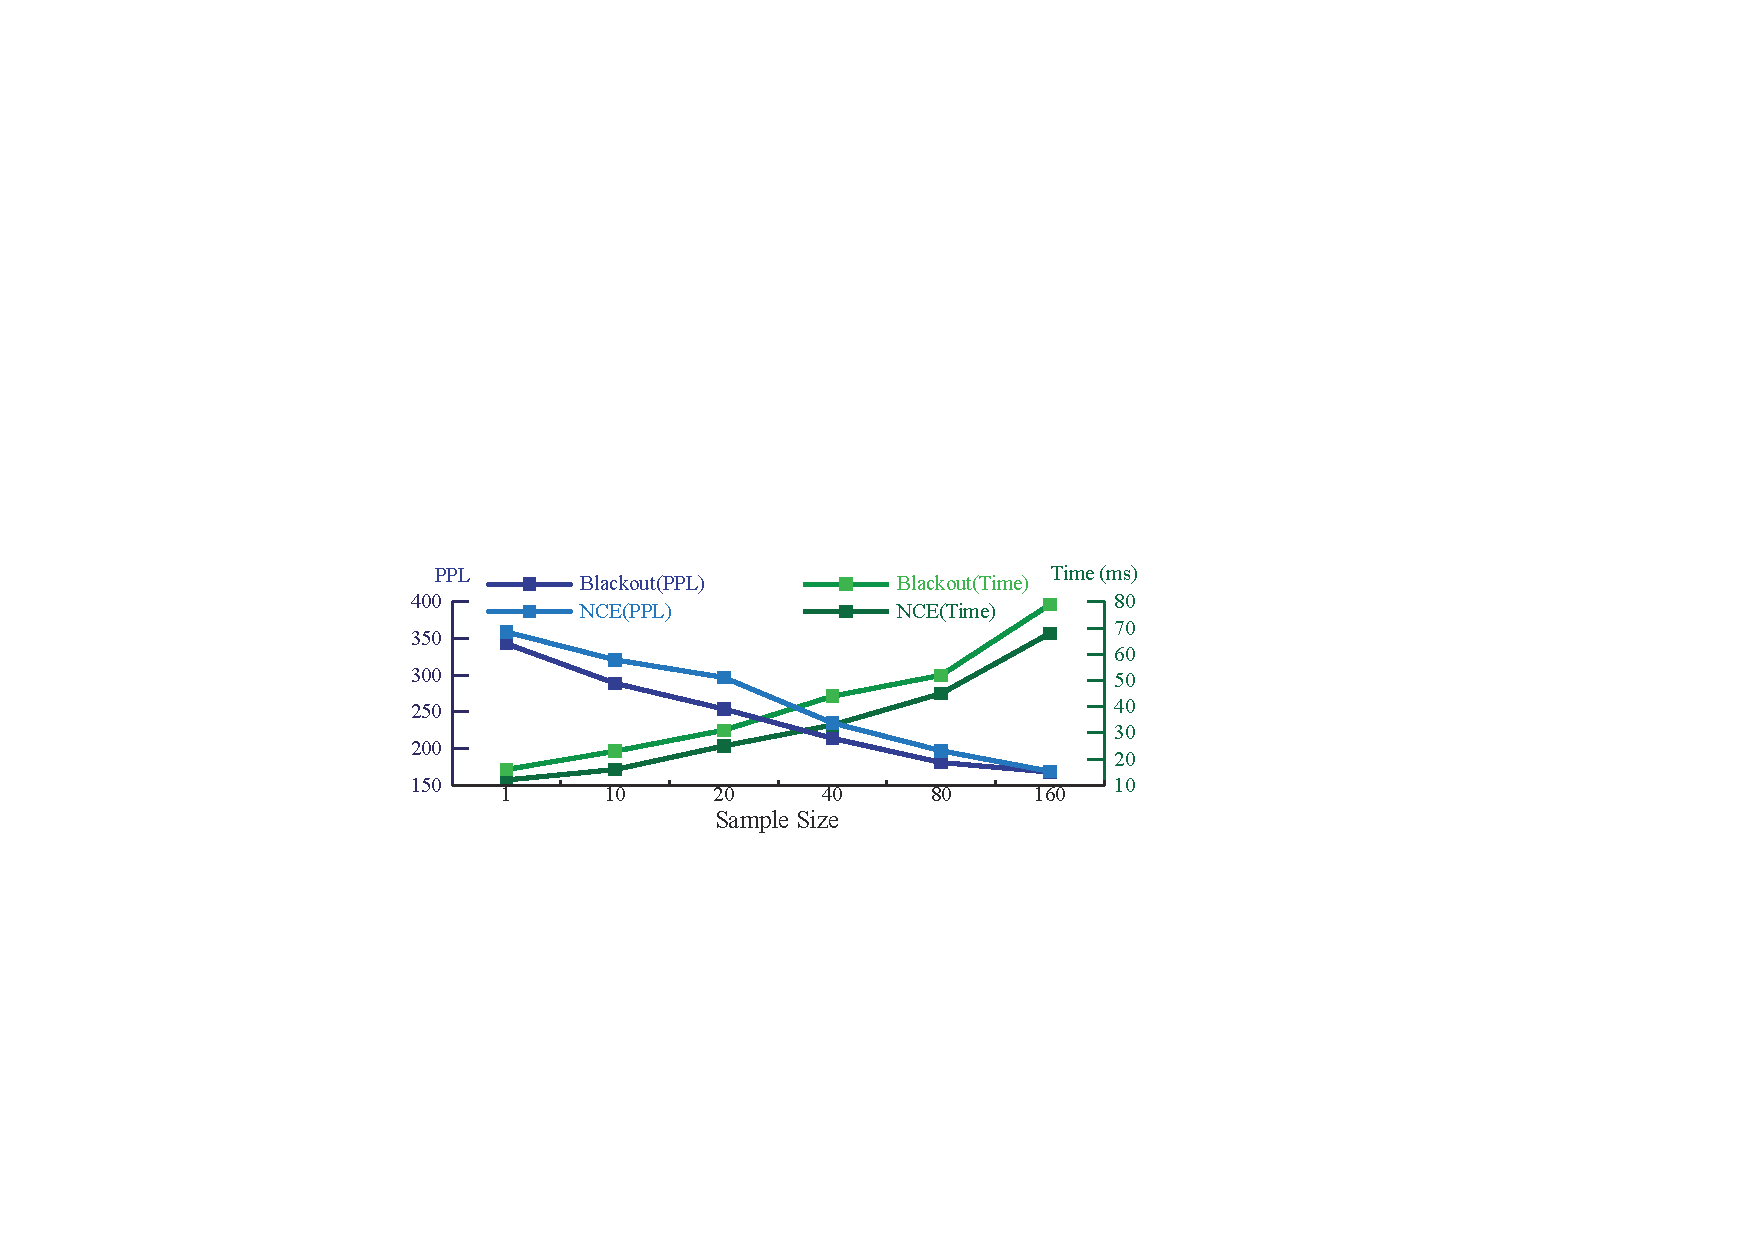
\includegraphics[width=.85\columnwidth]{./figures/nce_blackout.pdf}
  \caption{Wikitext-2上测试不同采样数量对NCE和Blackout算法的影响}\label{fig:blackout_nce}
\end{figure}


\subsection{单词聚类策略分析}
Chen~等人发现~cHSM~和~p-tHSM~算法的性能对不同单词的层次聚类算法很敏感~\upcite{DBLP:conf/acl/ChenGA16},因此为了获得较为稳定的~cHSM~算法和~p-tHSM~方法,本文考虑已有的聚类策略,结果展示在表~\ref{table:p-thsm}~和表~\ref{table:clustering}~中。

\begin{table}[!ht]
  \centering
   \caption{Wikitext-2上评价不同聚类方法对p-tHSM 算法的PPL影响\label{table:p-thsm}}
  \begin{tabular}{lcccc} \toprule
  算法  &建树时间&最大树深度 &验证集 (PPL) & 测试集 (PPL)  \\ \midrule
  Uni-gram  &3分钟&12 &218.42& 216.05     \\
  Bi-gram  &35小时&21& 186.23& 189.58\\
  Semantic &26小时 &18& \textbf{163.12} & \textbf{178.78}\\
\bottomrule
  \end{tabular}
\end{table}

对于基于树的层次算法的初始化,我们采用了霍夫曼聚类、布朗聚类和词向量聚类三种方法来生成不同的单词分布,详细的结果展示在表~\ref{table:p-thsm}~中。与能调整分支因子数目的~cHSM~方法不同,p-tHSM~算法由于子树最后都合并到根节点,所以不需要调整分支因子数。从实验结果中分析得知,一方面Uni-gram~聚类方法在创建单词层次结构方面效率最高,而~Bi-gram~和语义聚类需要花费巨额时间来计算词表中单词之间的相似度矩阵。另一方面,针对聚类的距离尺度,Uni-gram~以单词的词频为权重,Bi-gram~方法考虑二元共现单词的统计信息,语义聚类方法则计算特征空间中的两单词的余弦距离。在~PPL~指标比较中,采用~Bi-gram~和语义聚类的方法比采用霍夫曼聚类的方法拥有更低的分数。

\begin{table*}[!t]
\small
  \centering
  \caption{Wikitext-2数据集上不同聚类算法对cHSM 算法的PPL 和 WER 影响\label{table:clustering}}
  \begin{tabular}{lclccc} \toprule
聚类算法 & 均匀划分?&分支数& 训练轮数& 测试集 (PPL / WER)&耗时 (ms)\\ \midrule
  \multirow{6}{*}{Random}  &\multirow{6}{*}{是}&10/3330&145&211.15 / 78.55 &791\\
    &&20/1664&123&228.72 / 78.89&565\\
    &&40/832&103&234.36 / 79.21&321\\
    &&80/417&78&243.12 / 79.64&171\\
    &&160/208 &57&253.38 / 80.08&92\\
    &&182/183&48&268.63 / 80.11&88\\
  \midrule
  \multirow{6}{*}{Alphabet}  &\multirow{6}{*}{是}&10/3330 &141&199.01 / 78.07 &773\\
    &&20/1664 &120&211.34 / 78.23&551\\
    &&40/832 &100&238.75 / 79.02&313\\
    &&80/417 &90&241.75 / 79.34&174\\
    &&160/208 &56&248.35 / 79.62&97\\
    &&182/183&45&258.57 / 80.02&87\\
  \midrule
  \multirow{6}{*}{Uni-gram}   &\multirow{6}{*}{是} &10/3330&134&211.51 / 77.41 &788\\
    & &20/1664&122&220.01 / 77.71&549\\
    & &40/832&113&236.56 / 77.95&302\\
    & &80/417&91& 241.12 / 78.25&170\\
    & &160/208&55&247.25 / 79.21&93\\
    & &182/183&42&253.35 / 79.92&86\\
  \midrule
  \multirow{5}{*}{Bi-gram}   &\multirow{5}{*}{否}&10/3672&150&208.11 / 77.32&801\\
     &&20/1923&121&217,34 / 77.64&621\\
     &&40/1123&102&228.87 / 78.14&588\\
     &&80/572&89&246.32 / 78.43&186\\
     &&160/340&76&252.33 / 79.51&97\\
  \midrule
  \multirow{5}{*}{Syntactic}  &\multirow{5}{*}{否}&10/3612 &152&214.31 / 78.11&810\\
    &&20/1972 &130&220.19 / 78.86&633\\
    &&40/996 &101&232.33 / 79.33&543\\
    &&80/545 &89&241.34 / 79.84&179\\
    &&160/235 &70&262.34 / 80.14&134\\
  \midrule
  \multirow{5}{*}{Semantic}  &\multirow{5}{*}{否} &10/3570 &133&208.77 / 77.41&819\\
    & &20/1873 &114&218.31 / 77.78&641\\
    & &40/1092 &91&225.38 / 78.35&521\\
    & &80/561 &69&238.45 / 78.91&174\\
    & &160/244 &44&256.75 / 79.41&103\\
\bottomrule
  \end{tabular}
\end{table*}

表~\ref{table:clustering}~讨论了在~Wikitext-2~数据集上,cHSM~算法上应用前章节所介绍的不同聚类方法之间的差异,同时比较了不同的分支因子对算法效果的影响。从该表的结果分析得出,随机初始化方法性能最差,因为它没有提供有效的先验信息,从而干扰模型的学习过程。
此外还观察到,随机初始化的策略具有更大的训练误差需要更多的训练轮数来使之收敛。
然后,发现在对模型的类结构注入Uni-gram和Bi-gram的信息之后,模型能在特征空间学习到相对较好的单词分布。
因此,这两者比随机初始哈和按字母顺序初始化的算法在PPL和WER两种指标上结果更好。

而且,用语法和语义聚类算法将词表进行切分,能比其他的分割算法取得更好的PPL和WER数值。这间接表明,若能将有效的正确的知识注入模型的训练过程,模型理论上将获得更好的概率分布和更优良的稳定性。相比于二叉树层次概率模型,该算法还能动态调整分支因子,模型的适用范围相对更广。

\section{模型总体评价}
表~\ref{tab:summary_ppl}~统计了所有模型在上述三种标准语料的验证和测试数据集的PPL和WER结果。我们采用单层GRU单元作为这些算法的上下文表示,其维数设置为256。另外,对于~NCE~和~Blackout~采样算法,超参数~$k$~对较小的~Wikitext-2~和~Wikitext-103~数据集设置为$\mathcal{|V|}/20$,对于较大的~OBW~数据集设置为~$k=|\mathcal{V}|/200$。 此外,对于~cHSM~方法,我们根据单词的词频分布来划分词表。

\begin{table}[!t]
  \centering
  \caption{所有模型在三个数据集上的PPL和WER的性能评测\label{tab:summary_ppl}}
\begin{tabular}{llcc}
  \toprule
数据集& 算法& 验证集(PPL/WER) & 测试集(PPL/WER) \\ \midrule
 \multirow{2}{*}{WikiText-2}&GRU + Softmax&172.64 / 77.49\%&162.09 / 77.07\% \\
  &GRU + NCE~\cite{DBLP:journals/jmlr/GutmannH10}&217.84 / 78.26\%&199.54 / 78.02\%\\
  &GRU + Blackout~\cite{DBLP:journals/iclr/JiVSAD15}&221.15 / 77.72\%&199.56 / 77.50\% \\
  &GRU + cHSM + Uni-gram~\cite{DBLP:conf/acl/ChenGA16}&203.18 / 78.25\%&206.61 / 78.02\%\\
  &GRU + p-tHSM + Uni-gram~\cite{DBLP:conf/nips/MikolovSCCD13}&218.42 / 78.15\%&216.05 / 78.15\%\\
  &GRU + p-tHSM + Bi-gram~\cite{DBLP:journals/coling/BrownPdLM92}&186.23 / 78.15\%&189.58 / 78.15\%\\\midrule
   \multirow{2}{*}{WikiText-103} &GRU + Softmax&130.38 / 72.15\%&136.83 / 72.37\%\\
 &GRU + NCE~\cite{DBLP:journals/jmlr/GutmannH10}&164.78 / 73.22\%&165.01 / 73.34\%\\
  &GRU + Blackout~\cite{DBLP:journals/iclr/JiVSAD15}&163.99 / 73.18\%&162.76 / 74.22\%\\
  &GRU + cHSM + Uni-gram~\cite{DBLP:conf/acl/ChenGA16}&161.81 / 73.42\%&156.74 / 73.18\%\\
  &GRU + p-tHSM + Uni-gram~\cite{DBLP:conf/nips/MikolovSCCD13}&165.70 / 73.53\%&166.11 / 72.44\%\\
  &GRU + p-tHSM + Bi-gram~\cite{DBLP:journals/coling/BrownPdLM92}&164.15 / 78.15\%&163.55 / 77.85\%\\\midrule
  \multirow{2}{*}{One Billion Words} &GRU + Softmax&330.38 / 88.15\%&330.83 / 88.37\%\\
 & GRU + NCE~\cite{DBLP:journals/jmlr/GutmannH10}&272.07 / 84.83\%&276.11 / 84.34\%\\
  &GRU + Blackout~\cite{DBLP:journals/iclr/JiVSAD15}&268.67 / 84.23\%&266.11 / 84.18\%\\
 & GRU + cHSM + Uni-gram~\cite{DBLP:conf/acl/ChenGA16}&225.36 / 80.32\%&224.11 / 79.42\%\\
 & GRU + p-tHSM + Uni-gram~\cite{DBLP:conf/nips/MikolovSCCD13}&231.44 / 87.53\%&236.11 / 82.53\%\\
  %&GRU + p-tHSM + Bi-gram~\upcite{DBLP:journals/coling/BrownPdLM92}& 221.55 / 81.15\%&218.70 / 83.15\%\\
  \bottomrule
\end{tabular}
\end{table}

对于~Wikitext-2~数据集上的结果分析发现,softmax比其他算法的准确度更好,这是因为引入采样函数或者层次结构将会一定程度上加入人为的先验分布同时丢失了一部分信息,这妨碍了模型的训练收敛过程。

对于第二个Wikitext-103数据集,基于布朗聚类的p-tHSM方法获得了比霍夫曼聚类方法更好的PPL值和WER结果,另外布朗聚类用于初始化cHSM模型也能获得很好的准确率结果。由于Wikitext-103和Wikitext-2数据集共享相同的测试集,因此发现模型在大数据集上可以收敛到更好的结果 ,这证明了添加训练数据是一种提高模型的精度的有效途径。此外,对于采样算法的收敛结果比softmax方法好得多,同时提高了时间效率。
\section{本章小结}
本章首先定量分析了大词表问题,接下来比较了本文提出的层次概率模型的计算效率和传统算法之间的差异。针对层次模型的初始化算法,我们讨论并评估三种不同的层次聚类算法,以更有效的方式组织结构化的词表。结果表明,与其他概率归一化方法相比,本文提出的层次概率算法具有很好的计算速度提升效果。同时还讨论了两种层次概率模型的适用范围和两者的优缺点。
%在未来的研究中,我们计划探索softplus函数的应用场景,并探讨在cHSM算法训练的时候的词表动态交换算法。另外,实验中应用的几种聚类算法消耗了很多时间,我们可以优化该聚类算法,设计更高效的分层结构。
